% Section 1 pages 601 -
% \documentclass{article}
% % List all of the packages used in all of the files, which can the just be added as an input.
\usepackage[margin=1in]{geometry}
\usepackage{titlesec}
\usepackage{amsmath}
\usepackage{subfiles}
\usepackage{mathptmx}
\usepackage{csvsimple-l3}
\usepackage[T1]{fontenc}
\usepackage[utf8]{inputenc}
\usepackage{tabularx,ragged2e,booktabs,caption}
\usepackage{tikz}
\usepackage[colorlinks=true,allcolors=blue]{hyperref}
\usepackage{graphicx}
\usepackage{changepage}
\usepackage{natbib}
\usepackage{longtable}
\usepackage{abstract}
\usepackage{atbegshi}% http://ctan.org/pkg/atbegshi
% LaTeX path to the root directory of the current project, from the directory in which this file resides
% and path to econtexPaths which defines the rest of the paths like \FigDir
\providecommand{\econtexRoot}{}\renewcommand{\econtexRoot}{..}
\providecommand{\econtexPaths}{}\renewcommand{\econtexPaths}{\econtexRoot/TeXtools/econtexPaths}
% Mimicing professor's "ugly" solution to enable sharing base code between local LaTeX compilation and Overleaf

\providecommand{\FigDir}{\econtexRoot/FigDir}
\providecommand{\DataDir}{\econtexRoot/Data}
\providecommand{\SectionDir}{\econtexRoot/Sections}
\providecommand{\AppDir}{\econtexRoot/Appendices}
\providecommand{\TablesDir}{\econtexRoot/Tables}

\documentclass[\econtexRoot/ImaiKeane]{subfiles}
%\onlyinsubfile{\externaldocument{\econtexRoot/ImaiKeane}}

\begin{document}

\section{INTRODUCTION}
\label{section:intro}
\quad The intertemporal elasticity of substitution in labor supply (i.e.s.) has been a topic of considerable interest in both labor and macroeconomics for at least the past 30 years (see, e.g.,\cite{Lucas1969-ti}). Recently, there have been several studies that address the question using micropanel data. Classic examples are \cite{MaCurdy1981-iy}, \cite{Browning1985-ox}, and \cite{Altonji1986-zf}. They focus on estimating the intertemporal elasticity of substitution in labor supply, using marginal utility of wealth constant labor supply functions. In their work they assume that the utility function is time separable and wages are exogenous.\par
But if current labor supply leads to human capital accumulation (i.e., learning by doing), then estimates of the i.e.s. under a false assumption of no human capital accumulation are likely to be biased towards zero. The reason is as follows: As the wage increases over the life cycle, the substitution effect induces labor supply to increase, thus providing an incentive for people to supply more labor in older age. On the other hand, both concavity of the value function with respect to human capital and the approaching retirement period lower the marginal rate of return to human capital investment, thus reducing the incentive to supply labor. If these two factors roughly cancel, then even if wages increase over the life cycle, labor supply will be little changed (see Figure \ref{fig:OptimalSupply}). If we only allow for the substitution effect and not the human capital effect, the i.e.s. is identified primarily from the covariation of the wages and hours over the life cycle. Then, we will falsely conclude that the i.e.s. is low, simply because labor supply remains roughly constant over the life cycle even though wages increase\footnote[2]{ \cite{Heckman1976-lc} makes a similar point in the context of a model where workers choose the fraction of time on the job to devote to investment in human capital (in contrast to our learning-by-doing setup). Since workers are only paid for time spent in production, "measured wage rates obtained by dividing weekly income by weekly reported hours on the job systematically understate the true wage rate." This understatement of the "true wage rate" (or opportunity cost of time) is greatest at younger ages. Thus, over the life cycle the opportunity cost of time is flatter than the wage rate}. \par
% Drawing figure 1, illustration of life cycle labor supply
%\hypertarget{OptimalSupply}
\begin{figure}[tbp]
 \centerline{
  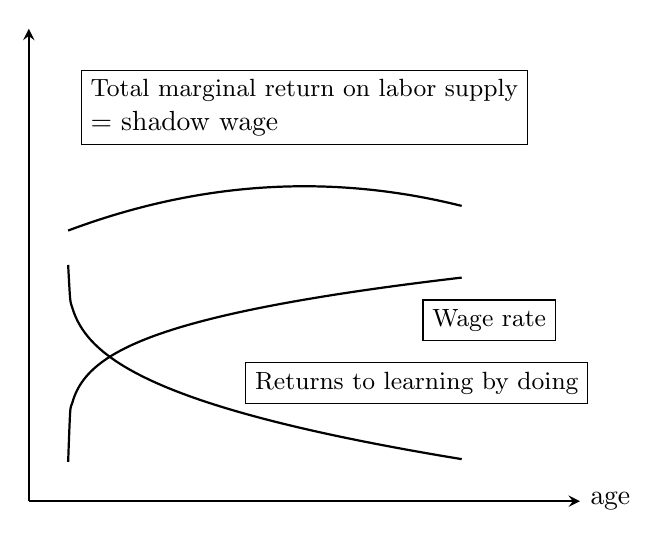
\begin{tikzpicture}
\draw[-stealth, black, thick] (0,0) -- (7,0) node[right] { age};
\draw[-stealth, black, thick] (0,0) -- (0,6);
\draw[thick, smooth, samples=200, xshift=.5cm, yshift=.5cm, domain=0:5] plot ({ \x, {(6*\x)^(1/4)}});
\node[right] at (5,2.3) [rectangle,draw] {\small Wage rate};
\draw[thick, smooth, samples=200, xshift=.5cm, yshift=3cm, domain=0:5] plot ({ \x, {-(3*\x)^(1/3)}});
\node[right] at (2.75,1.5) [rectangle,draw] {\small Returns to learning by doing};
% \draw[thick, smooth, samples=200, xshift=.5cm, yshift=2.5cm, domain=0.05:2.05] plot ({ \x, {\x^(1/2)-\x^(1/3)}});
\draw[thick, smooth, samples=200, xshift=-.5cm, yshift=2cm, domain=1:6] plot ({ \x, {2-(\x/4 - 1)^2}});
\node[align=left] at (3.5,5) [rectangle,draw] {\small Total marginal return on labor supply \\ = shadow wage};
\end{tikzpicture}
}
\caption{OPTIMAL LIFE CYCLE LABOR SUPPLY}
\label{fig:OptimalSupply}
\end{figure}
In this article, we address the issue of human capital accumulation in two steps. First, we estimate the life cycle labor supply model using maximum likelihood (ML) estimation based on a full solution of agents' dynamic programming problem that allows human capital accumulation. In the estimation, we use the white male sample in the NLSY79 data (see Section 5). Our estimate of the disutility of labor or parameter implies that the i.e.s. is 3.82, which is quite comparable to results obtained and used in the macroliterature. What drives this result is that once human capital is included in the model, the i.e.s. is identified off the covariation of hours with the opportunity cost of time (not just the wage rate). Since the life cycle pattern of the opportunity cost of time is fairly flat, the i.e.s. is identified primarily off of short-run covariation between hours and wages. \par
In the second step, we simulate data from the estimated model. Using the simulated data, we estimate consumption and labor supply Euler equations like those in  \cite{MaCurdy1981-iy} and \cite{Altonji1986-zf}, which do not allow for human capital accumulation. The elasticity estimates we obtain from the simulated data using the MaCurdy estimation method range from 0.3 to 1.1 when we use all the simulated data, and from 0.1 to 1.7 after we remove the outliers from the simulated data using a similar procedure to \cite{MaCurdy1981-iy}. The elasticity estimates obtained using the consumption and labor supply data as in  \cite{Altonji1986-zf} range from -0.2 to 2.8. These estimates are significantly lower than the ML estimate. OLS and IV results from the NLSY97 data are also reported and the i.e.s. is again estimated to be low. \par
The high elasticity obtained by full solution estimation, and the contrasting low elasticities implied by the conventional estimation methods imply that the latter are significantly biased towards zero, and that one of the main reasons behind this is the omission of human capital accumulation. Thus, our results may explain the apparent contradiction between the macro- and microliterature noted above. \par
Notice that in conventional methods of estimation such as \cite{MaCurdy1981-iy} or  \cite{Altonji1986-zf}, the i.e.s. is defined and estimated as the elasticity of substitution when workers change labor supply along the anticipated life cycle wage path. But in macroeconomics, the discussion is typically about how labor supply responds to unanticipated business cycle shocks. In our analysis, we explicitly solve the dynamic programming model including unanticipated wage shocks. Therefore, our estimate is more relevant in providing microevidence for use in calibrating real business cycle models. After the estimation, we also simulate the hours response to a temporary 2\% increase in the rental rate on human capital. There, we show that even though the elasticity of labor supply is 3.82, this does not imply that hours increase by roughly 4 times the percentage amount of the wage increase. Rather, although such a large response is observed for older workers, the response for young workers is much smaller. This is because of the role of human capital accumulation, which we discuss more later \footnote[3]{Recently, several authors, such as \cite{Cooper1999-af} or \cite{Chang2002-zs}, have introduced learning by doing (LBD) into the standard real business cycle model as an internal propagation mechanism. \cite{Cooper1999-af} assume LBD in organizational capital at the plant level and \cite{Chang2002-zs} assume LBD in the human capital accumulation of workers over the life cycle. Their models succeed in generating persistence in macroeconomic variables even though their underlying technology shocks are set to be uncorrelated over time. Furthermore, their calibrated impulse-response function of output has the familiar hump-shaped form seen in the U.S. GDP time series data. Since the agents in our model are very similar to those assumed by \cite{Chang2002-zs}, our article provides some empirical evidence supporting the above line of research.}. \par
The theory of optimal life-cycle consumption and labor supply with human capital accumulation has been developed by \cite{Heckman1976-lb} and \cite{Heckman1976-lc}, \cite{Ben-Porath1967-sf}, \cite{Blinder1976-dv}, and others. They provide a neoclassical theoretical framework to explain the life-cycle profiles of wages, schooling, and work hours. \cite{Shaw1989-jb} was among the first to estimate a dynamic labor supply model that includes human capital accumulation. \cite{Shaw1989-jb} estimated Euler equations of optimal consumption and labor supply using the nonlinear GMM method. But in her work, she used the translog utility function for consumption and labor supply hours. Hence, she did not explicitly estimate the i.e.s. parameter. \cite{Altug1998-ou} also estimate a dynamic labor supply model for females. \par
\cite{Eckstein1989-ji} also include human capital in a life cycle labor supply model that they estimate by ML. But they restrict labor hours to two categories: zero hours or full time. If people intertemporally substitute labor but still stay within the same broad hours classification, their estimate of the i.e.s. may be downwardly biased. But if most people work around the borders of the two categories, then small changes in labor supply will be classified as changes between two categories; thus the i.e.s. will be overestimated. Since the former case seems to be more likely in a discrete choice model of labor supply, we suspect that one is likely to get downwardly biased estimates of the i.e.s.. Also, since they use a linear utility function for consumption, there is no wealth effect in their model, even though the wealth effect may be an important factor linking peoples' decisions intertemporally. \cite{Keane2001-yk} estimate a model with human capital accumulation and saving, but hours are also discrete in their model (e.g., full time, part time, and zero hours work). \par
The major obstacle to ML estimation of the dynamic labor supply model with continuous hours and human capital accumulation is that the full solution of the continuous variable dynamic programming problem implied by this model is extremely computationally demanding. There are two reasons. First, the state space of the dynamic programming problem is now infinite. Even in a discrete choice dynamic programming problem, where there is only a finite state space, researchers are usually plagued with the problem of having too many state space points to evaluate the value function (see, e.g., \cite{Geweke2001-px}; \cite{Keane1994-sm}). In the continuous choice case, explicit evaluation of the value function at each state space point is impossible. Second, in contrast to a discrete choice dynamic programming problem where solving for the control variables is a trivial optimization over a finite set of choices, in the continuous choice problem, solving for the control variables is the main source of computational burden. It requires a two-dimensional nonlinear Newton search algorithm to find optimal consumption and labor supply at each state space point. \par
Here we develop an algorithm that approximates the solution to the DP problem. The algorithm successively solves the Bellman equation backwards from the last period. First, we choose a finite set of grid points over assets and human capital at which to evaluate the expected value function (emax function). The emax function derived above is used for the next Bellman backward iteration. The main feature of the algorithm is that we avoid two-dimensional quadrature integration over both taste shocks and wage shocks by exploiting the fact that there is a one-to-one mapping from human capital to wages. Reducing the dimensionality of quadrature integration decreases the number of computationally demanding Newton searches by an order of magnitude. Also, by reducing the range of human capital points at which the value functions must be evaluated, it makes the Newton search algorithm itself easier and more accurate. \par
We apply our model to white males from the 1979 youth cohort of the National Longitudinal Survey of Labor Market Experience (NLSY79). Among the features of the NLSY79, which distinguishes it from the commonly used Panel Study of Income Dynamics (PSID), is detailed asset data for individuals from 1985. Instead of using food consumption to derive the marginal value of wealth at some period, which is commonly done by researchers using the PSID, we use asset data directly. We then derive total consumption by using the asset data and the intertemporal budget constraint. \par
The organization of the article is as follows. Section \ref{section:model} presents the model, Section \ref{section:solving} describes the algorithm for solving the DP problem, and Section \ref{section:MLE} describes the algorithm for forming the likelihood function. Section \ref{section:data} describes the data, and Section \ref{section:estimation} discusses the estimates and some model simulations. Section \ref{section:conclusions} concludes.
\end{document}
